% !TEX TS-program = xelatex
% !TEX encoding = UTF-8 Unicode
% !Mode:: "TeX:UTF-8"

\documentclass{resume}
\usepackage{zh_CN-Adobefonts_external} % Simplified Chinese Support using external fonts (./fonts/zh_CN-Adobe/)
%\usepackage{zh_CN-Adobefonts_internal} % Simplified Chinese Support using system fonts
\usepackage{graphicx} % 插入图片的宏包
\usepackage[absolute,overlay]{textpos} % 允许在页面的绝对位置放置内容
\usepackage{linespacing_fix} % disable extra space before next section
\usepackage{cite}

\begin{document}
\pagenumbering{gobble} % suppress displaying page number

% 在页面的右上角插入照片
\begin{textblock*}{30mm}(150mm,3mm) % 调整这里的坐标 (x,y) 和大小 (宽度)
  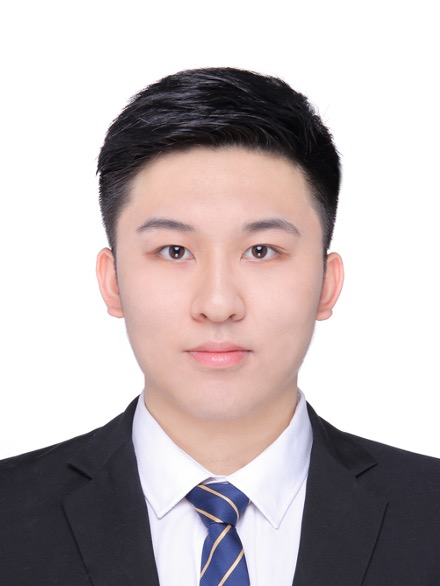
\includegraphics[width=30mm]{head_photo.jpg} % 照片的文件名
\end{textblock*}


\name{安澜霆 Amber}

% {E-mail}{mobilephone}{homepage}
% be careful of _ in emaill address
\contactInfo{(+86) 156-1118-7755}{532389813@qq.com}{中共党员}

% {E-mail}{mobilephone}
% keep the last empty braces!
%\contactInfo{xxx@yuanbin.me}{(+86) 131-221-87xxx}{}

\section{教育背景}
\datedsubsection{\textbf{清华大学},工业工程,\textit{在读硕士}}{2022.9 - 2025.6}
\datedsubsection{\textbf{复旦大学},软件工程,\textit{本科}}{2015.9 - 2019.6}
\ \textbf{复旦大学三等奖奖学金},团学联体育部副部长

%***********职业经历*********************
\section{职业经历}

\datedsubsection{\textbf{OKX Group},Web3合约组,智能合约高级开发工程师}{2022.04 - 2024.08}
\begin{itemize}[parsep=0.5ex]
  \item 主导设计并开发多链\textbf{NFT 聚合器和二级市场}智能合约,推动流动性聚合与功能迭代;
  \item 负责 Create Studio 2.0 与相关运营活动的合约架构设计与开发;
  \item 主导制定了预执行错误交易排查流程,并于多个团队推行;
  \item 组织内部技术分享、新人技术培训、wiki管理等团队管理工作;
  \item 负责行业内新技术、新趋势调研并推进落地产品化应用;
\end{itemize}

\datedsubsection{\textbf{中国外运},运营及数字化部,技术经理}{2021.10 - 2022.03}
\begin{itemize}[parsep=0.5ex]
  \item 与各部门协调,为各部门提供信息技术支持并对全公司的信息资源进行管理和控制;
  \item 根据企业发展战略和信息化战略要求,负责企业内外部信息资源开发利用;
  \item 参与公司信息化建设的总体规划及架构设计,建立企业信息化管理制度和标准规范;
\end{itemize}

\datedsubsection{\textbf{中国外运},工程技术部,Java开发工程师}{2019.08 - 2021.10}
\begin{itemize}[parsep=0.5ex]
  \item 荣获外运2019年度最佳管培生称号
  \item \textbf{HS 编码智能归类系统}:基于springboot框架,elasticsearch,mysql开发HS编码智能归类系统。其中负责代码架构搭建、基本功能开发、索引设计、数据库设计以及功能优化,jenkins 构建 CI/CD 流程,将项目构建为docker进行部署。
  \item \textbf{智慧工程物流系统}:基于springboot框架开发智慧工程物流系统。其中负责基本功能开发、数据库设计以及功能优化。使用 elasticsearch、logstash、kibana 搭建系统日志管理系统,保证系统的管理要求。
\end{itemize}

\datedsubsection{\textbf{上海复星杏脉科技},QT 开发工程师}{2019.02 - 2019.05}
\begin{itemize}[parsep=0.5ex]
  \item 8孔呼吸道病毒桌面挂件工具:使用 QT 开发平台,开发8孔呼吸道病毒数据显示桌面挂件工具。其中主要实现:多进程实现 QT c++与 python 算法(tensorflow-gpu)联调、多线程实现 QTc++ 与 python 功能函数联调。
\end{itemize}

%***********项目经历*********************
\section{项目经历}
\datedsubsection{\textbf{NFT Lending},智能合约工程师}{2021.06 - 2022.06}
\begin{itemize}[parsep=0.5ex]
  \item 基于 Solidity、Openzeppelin 实现 Dapp 的智能合约签名验证、收益计算等合约功能;
  \item 使用 Hardhat 对合约功能进行单元测试和流程测试,并将合约部署至 Rinkeby;
  \item 编写 Subgraph mapping script,将 event 数据索引至项目的 the graph 节点;
  \item 使用 Slither 检查合约代码中的 bad smell 并进行修复;
\end{itemize}
\datedsubsection{\textbf{}无人机巡检管理系统}{2019.09 - 2021.05}
\begin{itemize}[parsep=0.5ex]
  \item 负责系统整体模块与功能设计、数据库设计及机库管理、恶劣天气预警模块的开发;
  \item 使用 Websocket 实现无人机与系统的实时通信,并接入第三方地图服务显示无人机实时位置与信息;
\end{itemize}
\end{document}
